\chapter{Zakłócenie sinusoidalne}
W celu sprawdzenia wpływu zakłócenia sinusoidalnego na jakość regulacji (z pomierem i bez pomiaru) wygenerowane zostały przebiegi z zakłóceniami o różnej częstotliwości i różnej amplitudzie. Sygnałem zakłócający generowany był jako
\begin{equation}
	z = sin(k/p)*a
	\label{eq:zaksin}
\end{equation}
gdzie $p$ przybierało wartości:
\begin{itemize}
	\item $p=5$,
	\item $p=10$,
	\item $p=20$,
\end{itemize}
natomist $a$:
\begin{itemize}
	\item $a=0.1$,
	\item $a=0.2$,
	\item $a=1$.
\end{itemize}
Tak przygotowane wykresy można obejrzeć poniżej.
\begin{figure}[h!]
	\centering
	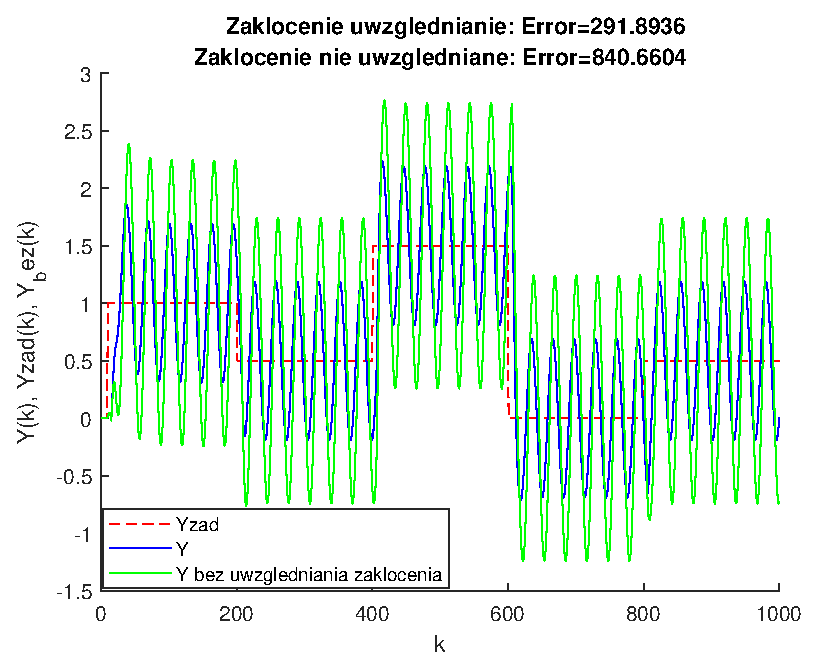
\includegraphics[scale=1]{Rys/sin5_1}
	\label{fig:sin5_1}
	\caption{Przebieg dla zakłócenia z parametrami $p=5$ oraz $a=1$}
\end{figure}
\begin{figure}[h!]
	\centering
	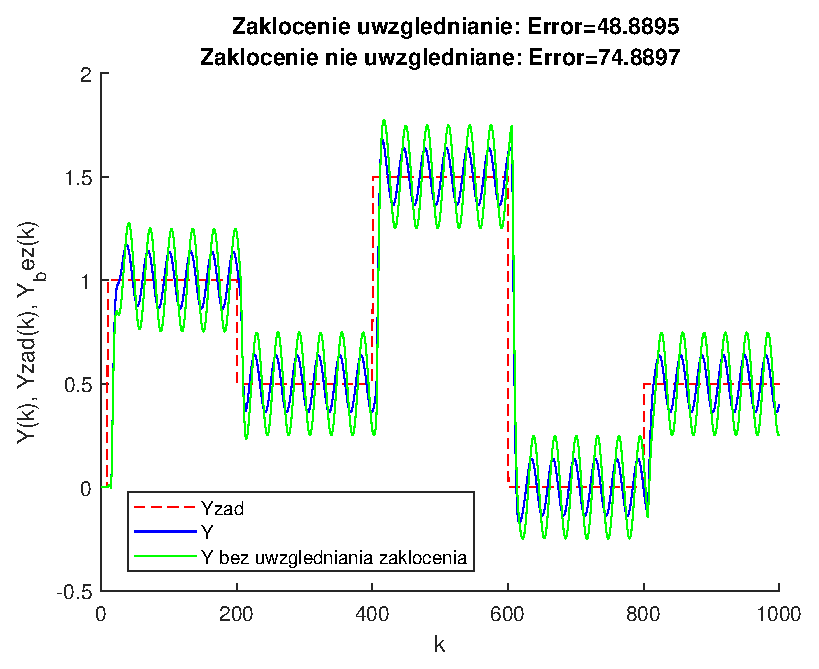
\includegraphics[scale=1]{Rys/sin5_5}
	\label{fig:sin5_5}
	\caption{Przebieg dla zakłócenia z parametrami $p=5$ oraz $a=0.2$}
\end{figure}
\begin{figure}[h!]
	\centering
	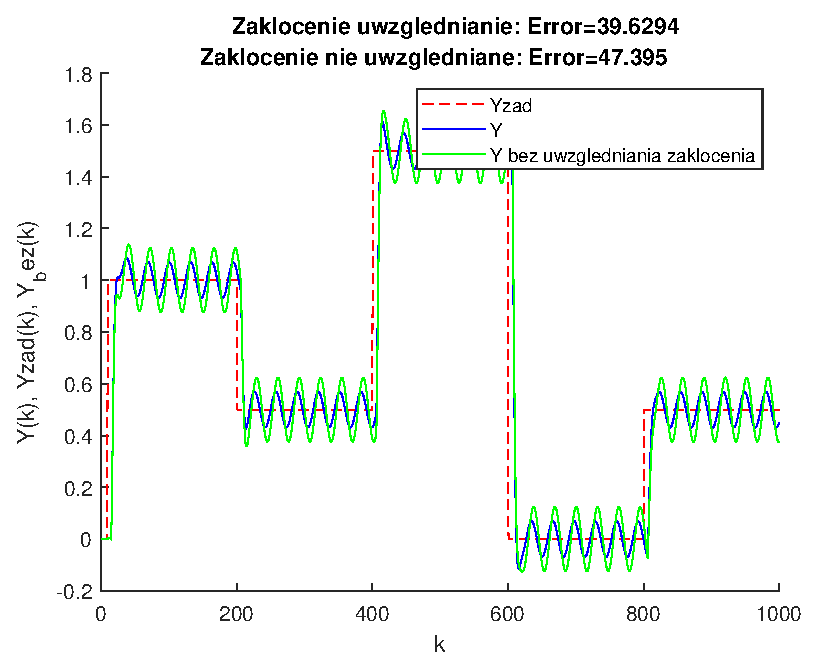
\includegraphics[scale=1]{Rys/sin5_10}
	\label{fig:sin5_10}
	\caption{Przebieg dla zakłócenia z parametrami $p=5$ oraz $a=0.1$}
\end{figure}
\begin{figure}[h!]
	\centering
	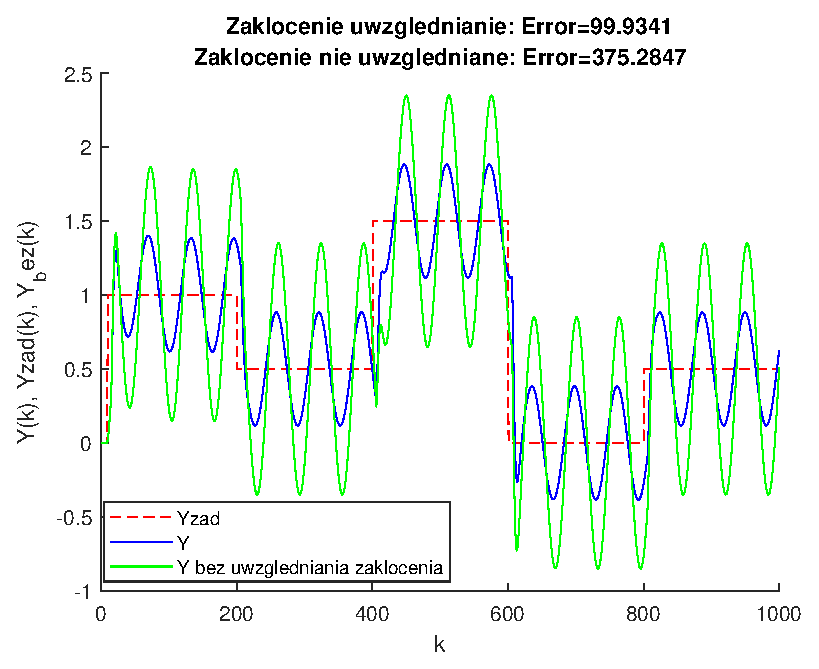
\includegraphics[scale=1]{Rys/sin10_1}
	\label{fig:sin10_1}
	\caption{Przebieg dla zakłócenia z parametrami $p=10$ oraz $a=1$}
\end{figure}
\begin{figure}[h!]
	\centering
	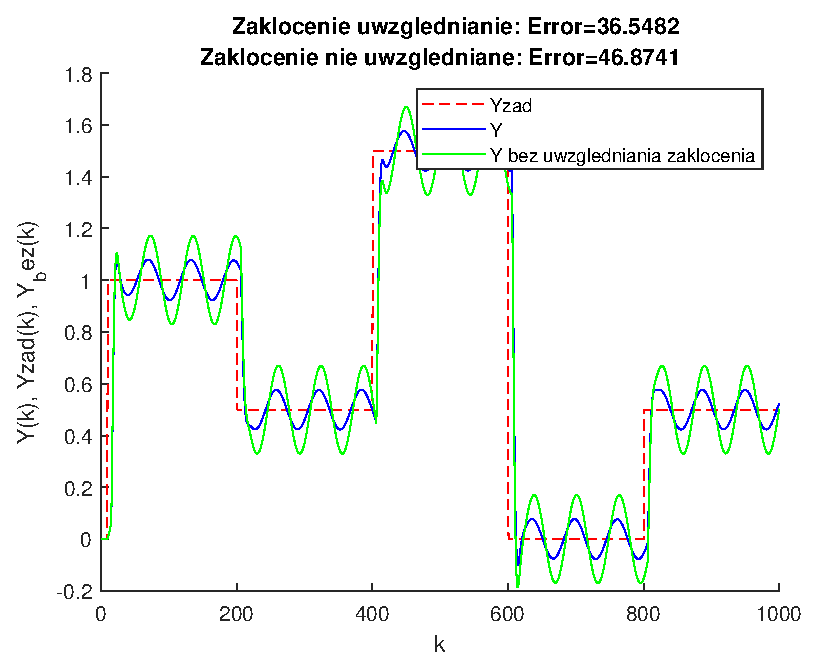
\includegraphics[scale=1]{Rys/sin10_5}
	\label{fig:sin10_5}
	\caption{Przebieg dla zakłócenia z parametrami $p=10$ oraz $a=0.2$}
\end{figure}
\begin{figure}[h!]
	\centering
	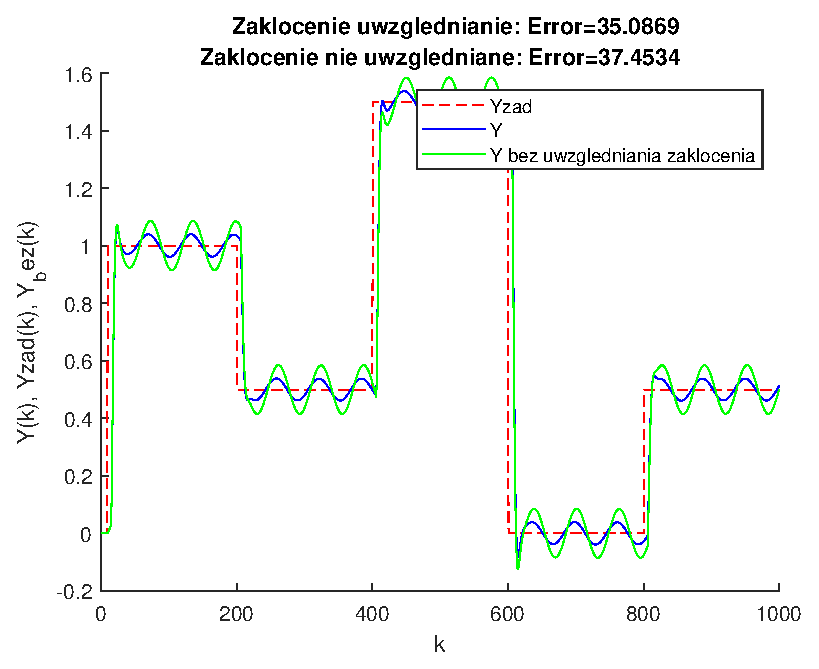
\includegraphics[scale=1]{Rys/sin10_10}
	\label{fig:sin10_10}
	\caption{Przebieg dla zakłócenia z parametrami $p=10$ oraz $a=0.1$}
\end{figure}
\begin{figure}[h!]
	\centering
	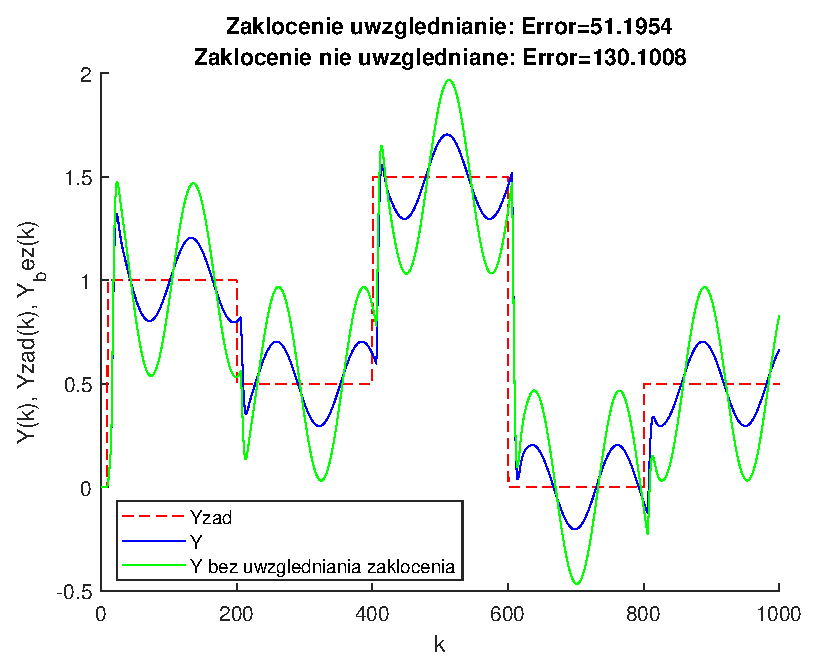
\includegraphics[scale=1]{Rys/sin20_1}
	\label{fig:sin20_1}
	\caption{Przebieg dla zakłócenia z parametrami $p=20$ oraz $a=1$}
\end{figure}
\begin{figure}[h!]
	\centering
	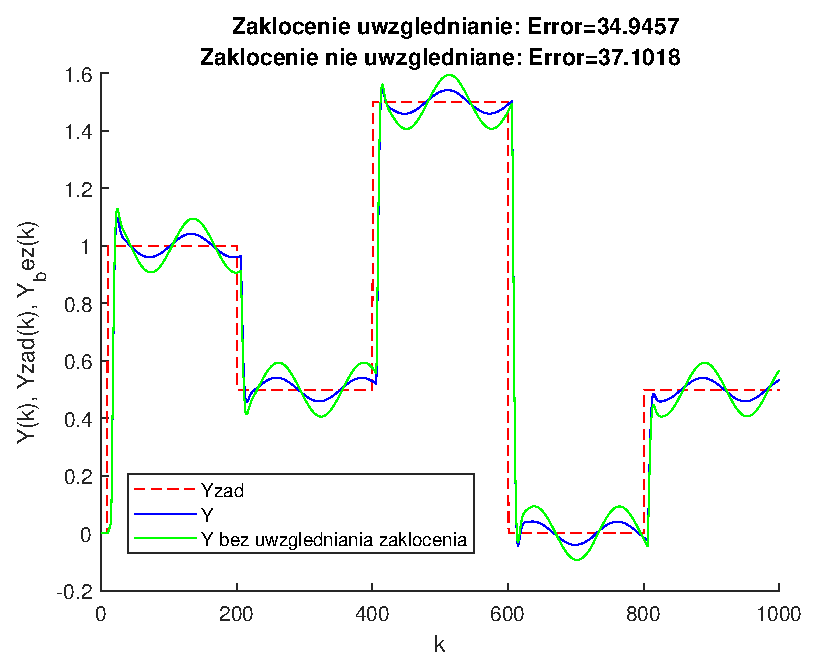
\includegraphics[scale=1]{Rys/sin20_5}
	\label{fig:sin20_5}
	\caption{Przebieg dla zakłócenia z parametrami $p=20$ oraz $a=0.2$}
\end{figure}
\begin{figure}[h!]
	\centering
	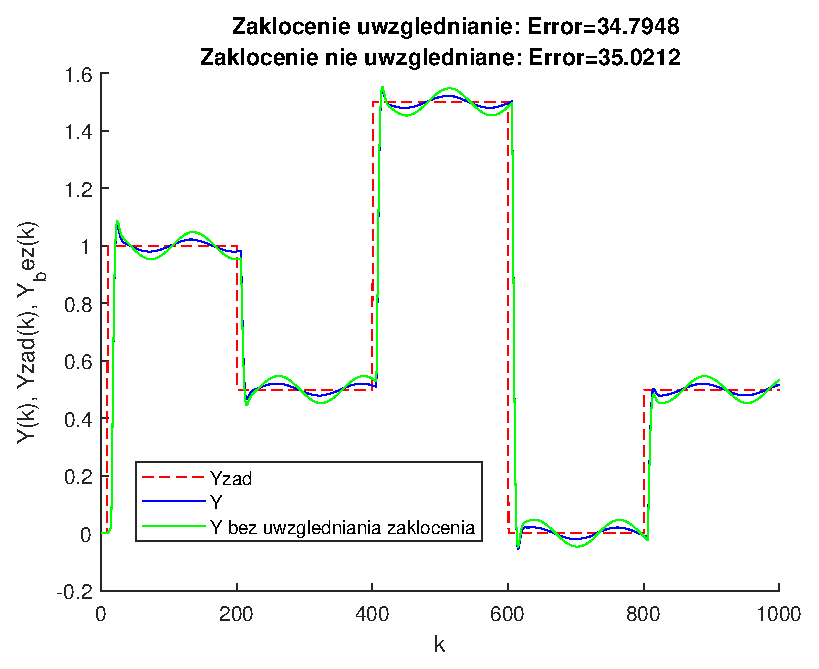
\includegraphics[scale=1]{Rys/sin20_10}
	\label{fig:sin20_10}
	\caption{Przebieg dla zakłócenia z parametrami $p=20$ oraz $a=0.1$}
\end{figure}